\documentclass[12pt,a4paper]{article}
\usepackage[utf8]{inputenc}
\usepackage[T1]{fontenc}
\usepackage[brazilian]{babel}
\usepackage{lmodern}
\usepackage{graphicx}
\usepackage{geometry}
\usepackage{fancyhdr}
\usepackage{booktabs}
\usepackage{longtable}
\usepackage{array}
\usepackage{float}
\usepackage{hyperref}

\geometry{margin=2.5cm}
\setlength{\headheight}{14.5pt}
\pagestyle{fancy}
\fancyhf{}
\rhead{Análise de Risco}
\lhead{Lista 4}
\cfoot{\thepage}

\title{\Large \textbf{Análise de Risco -- Lista 4} \\
       \large Risco de Prazo e Caminho Crítico}
\author{Grupo 6\\Bruna Irene da Silva (119062418)\\Davi dos Santos Mattos (119133049)\\Gabriel Mayrink Verdun (125078427)}
\date{26 de maio de 2026}

\begin{document}

\maketitle

\begin{abstract}
Este relatório apresenta a análise de risco de prazo de uma rede de projeto com 14 atividades, seguindo o método de Monte Carlo pedido no enunciado da Lista 4. Foram estimadas a distribuição empírica da duração total do projeto, a probabilidade de cada atividade pertencer ao caminho crítico, a distribuição dos tempos de início mais cedo, um cronograma com 85\% de chance de ser cumprido e o diagrama de Gantt correspondente ao cronograma final.
\end{abstract}

\section{Introdução}

O objetivo deste trabalho é estudar um problema clássico de agendamento com incerteza nas durações das atividades. A rede do projeto é orientada por precedência, e cada atividade possui duração modelada por distribuição triangular conforme a Tabela 1 do enunciado. A partir dessas distribuições, o projeto foi simulado por Monte Carlo para estimar medidas de risco e apoiar a construção de um cronograma de menor duração com nível de confiança de 85\%.

\section{Metodologia}

Foram consideradas 14 atividades e 6 caminhos possíveis entre o início e o fim da rede. As durações foram amostradas como números inteiros pela regra \texttt{ceiling} aplicada à distribuição triangular, reproduzindo a lógica usada no script em R. A análise principal foi executada com 10.000 repetições.

Os caminhos da rede são:
\begin{itemize}
    \item 1 $\rightarrow$ 2 $\rightarrow$ 9 $\rightarrow$ 14;
    \item 1 $\rightarrow$ 3 $\rightarrow$ 5 $\rightarrow$ 10 $\rightarrow$ 12 $\rightarrow$ 13 $\rightarrow$ 14;
    \item 1 $\rightarrow$ 3 $\rightarrow$ 6 $\rightarrow$ 12 $\rightarrow$ 13 $\rightarrow$ 14;
    \item 1 $\rightarrow$ 3 $\rightarrow$ 7 $\rightarrow$ 11 $\rightarrow$ 12 $\rightarrow$ 13 $\rightarrow$ 14;
    \item 1 $\rightarrow$ 3 $\rightarrow$ 7 $\rightarrow$ 8 $\rightarrow$ 13 $\rightarrow$ 14;
    \item 1 $\rightarrow$ 4 $\rightarrow$ 8 $\rightarrow$ 13 $\rightarrow$ 14.
\end{itemize}

\newpage
\section{Resultados}

\subsection{Item 1 -- Duração total do projeto}

A duração total empírica do projeto foi obtida como o maior tempo entre os caminhos simulados em cada cenário. Os principais indicadores são mostrados na Tabela~\ref{tab:duracao_total}.

\begin{table}[H]
\centering
\caption{Resumo estatístico da duração total do projeto}
\label{tab:duracao_total}
\begin{tabular}{lr}
\toprule
\textbf{Medida} & \textbf{Valor} \\
\midrule
Mediana & 21,00 \\
Desvio padrão & 2,17 \\
Mínimo & 14,00 \\
Máximo & 29,00 \\
P85 & 24,00 \\
\bottomrule
\end{tabular}
\end{table}

Assim, um prazo de 24 unidades de tempo cobre aproximadamente 85\% dos cenários simulados.

\begin{figure}[H]
\centering
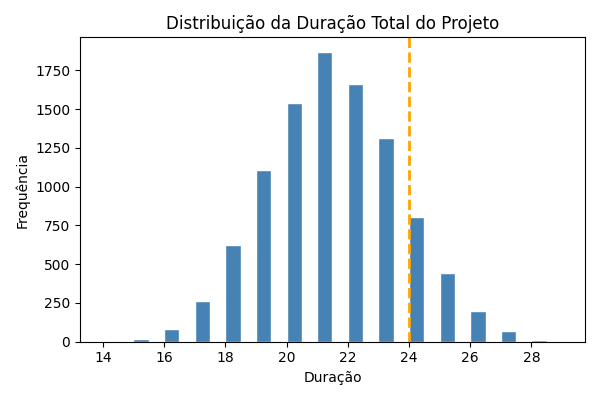
\includegraphics[width=0.8\textwidth]{durCC_hist.png}
\caption{Histograma da duração total do projeto}
\label{fig:dur_hist}
\end{figure}

\begin{figure}[H]
\centering
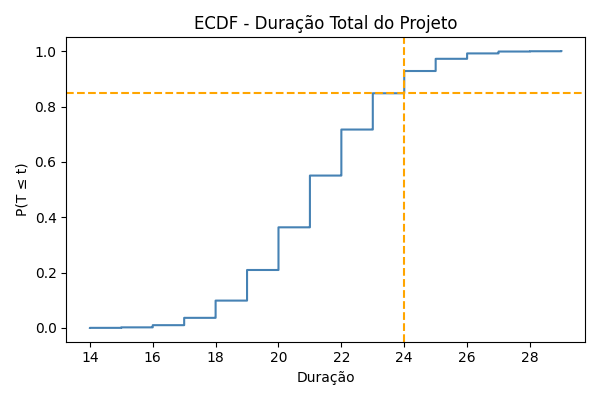
\includegraphics[width=0.8\textwidth]{durCC_ecdf.png}
\caption{ECDF da duração total do projeto}
\label{fig:dur_ecdf}
\end{figure}

\subsection{Item 2 -- Probabilidade de cada atividade estar no caminho crítico}

O caminho crítico não é fixo: ele varia conforme as durações sorteadas. A Tabela~\ref{tab:critico} resume a frequência empírica de cada atividade aparecer no caminho crítico.

\begin{table}[H]
\centering
\caption{Probabilidade empírica de cada atividade estar no caminho crítico}
\label{tab:critico}
\begin{tabular}{cr}
\toprule
\textbf{Atividade} & \textbf{Probabilidade (\%)} \\
\midrule
1 & 100,0 \\
2 & 0,0 \\
3 & 100,0 \\
4 & 0,0 \\
5 & 26,9 \\
6 & 66,4 \\
7 & 6,8 \\
8 & 0,0 \\
9 & 0,0 \\
10 & 26,9 \\
11 & 6,8 \\
12 & 100,0 \\
13 & 100,0 \\
14 & 100,0 \\
\bottomrule
\end{tabular}
\end{table}

As atividades 1, 3, 12, 13 e 14 aparecem em praticamente todos os cenários críticos, enquanto as atividades 5, 6, 7, 10 e 11 entram de forma dependente da combinação de durações sorteadas.

\begin{figure}[H]
\centering
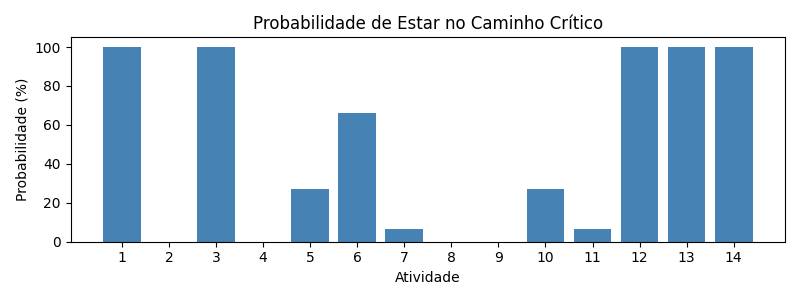
\includegraphics[width=0.9\textwidth]{probCC_bar.png}
\caption{Probabilidade de cada atividade estar no caminho crítico}
\label{fig:probcc}
\end{figure}

\subsection{Item 3 -- Distribuição dos inícios mais cedo}

Foram estimados, para cada atividade, a média, a mediana e o percentil 85 do tempo de início mais cedo. Esses valores mostram como a incerteza se propaga ao longo da rede.

\begin{longtable}{crrr}
\caption{Distribuição empírica dos inícios mais cedo por atividade}\label{tab:est}\\
\toprule
\textbf{Atividade} & \textbf{Média} & \textbf{P50} & \textbf{P85} \\
\midrule
\endfirsthead
\toprule
\textbf{Atividade} & \textbf{Média} & \textbf{P50} & \textbf{P85} \\
\midrule
\endhead
1 & 0,0 & 0,0 & 0,0 \\
2 & 0,0 & 0,0 & 0,0 \\
3 & 0,0 & 0,0 & 0,0 \\
4 & 0,0 & 0,0 & 0,0 \\
5 & 5,5 & 6,0 & 7,0 \\
6 & 5,5 & 6,0 & 7,0 \\
7 & 5,5 & 6,0 & 7,0 \\
8 & 8,3 & 8,0 & 10,0 \\
9 & 7,2 & 7,0 & 9,0 \\
10 & 7,2 & 7,0 & 9,0 \\
11 & 8,3 & 8,0 & 10,0 \\
12 & 12,6 & 13,0 & 14,0 \\
13 & 15,4 & 15,0 & 17,0 \\
14 & 21,3 & 21,0 & 24,0 \\
\bottomrule
\end{longtable}

\begin{figure}[H]
\centering
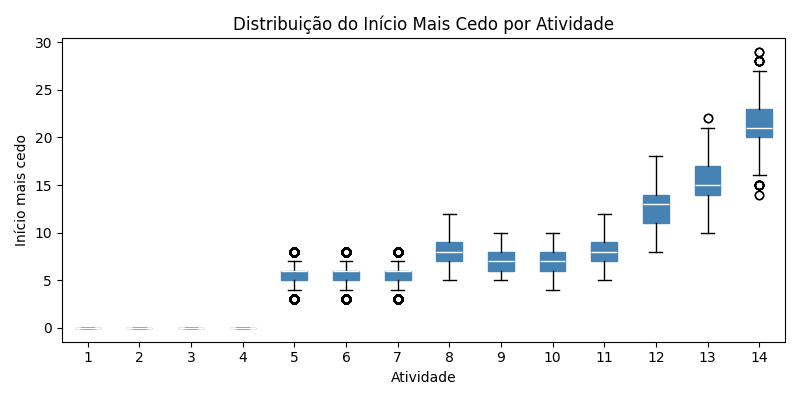
\includegraphics[width=0.9\textwidth]{est_boxplot.png}
\caption{Distribuição dos inícios mais cedo por atividade (boxplots)}
\label{fig:est_box}
\end{figure}

\subsection{Item 4 -- Cronograma com 85\% de chance de ser cumprido}

O cronograma final foi construído pela política de início mais cedo, usando os percentis 85\% dos inícios e das durações. O prazo total associado ao cronograma é 24 unidades de tempo.

\begin{table}[H]
\centering
\caption{Cronograma final com 85\% de chance de cumprimento}
\label{tab:cronograma}
\begin{tabular}{crrr}
\toprule
\textbf{Atividade} & \textbf{Início} & \textbf{Duração} & \textbf{Fim} \\
\midrule
1 & 0,0 & 0,0 & 0,0 \\
2 & 0,0 & 9,0 & 9,0 \\
3 & 0,0 & 7,0 & 7,0 \\
4 & 0,0 & 5,0 & 5,0 \\
5 & 7,0 & 2,0 & 9,0 \\
6 & 7,0 & 8,0 & 15,0 \\
7 & 7,0 & 4,0 & 11,0 \\
8 & 10,0 & 3,0 & 13,0 \\
9 & 9,0 & 5,0 & 14,0 \\
10 & 9,0 & 5,0 & 14,0 \\
11 & 10,0 & 3,0 & 13,0 \\
12 & 14,0 & 4,0 & 18,0 \\
13 & 17,0 & 7,0 & 24,0 \\
14 & 24,0 & 0,0 & 24,0 \\
\bottomrule
\end{tabular}
\end{table}

\subsection{Item 5 -- Diagrama de Gantt}

O diagrama de Gantt comum é obtido diretamente a partir do cronograma da Tabela~\ref{tab:cronograma}. Ele mostra as barras de execução de cada atividade, sem destaque especial para o caminho crítico, e é compatível com a política de início mais cedo usada no item anterior.

\begin{figure}[H]
\centering
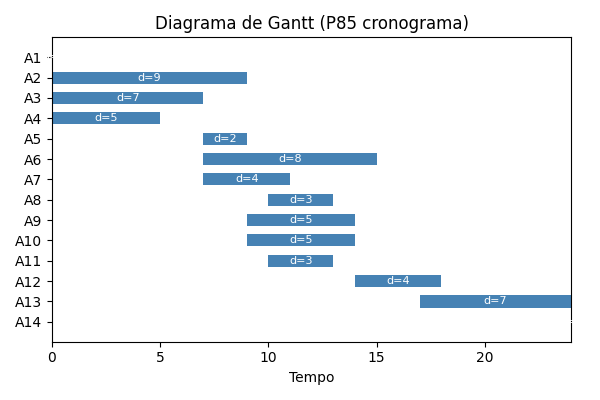
\includegraphics[width=0.9\textwidth]{gantt.png}
\caption{Diagrama de Gantt do cronograma P85}
\label{fig:gantt}
\end{figure}

\section{Conclusão}

A simulação de Monte Carlo permitiu quantificar a incerteza do prazo do projeto e identificar o comportamento do caminho crítico ao longo dos cenários. O prazo empírico estimado para 85\% de chance de cumprimento foi de 24 unidades de tempo. Além disso, as atividades 1, 3, 12, 13 e 14 apresentaram presença praticamente permanente no caminho crítico, indicando que elas concentram a maior sensibilidade da rede.

\end{document}